\documentclass[UTF8]{ctexart} %使用ctex包,中文支持
\usepackage{amsmath}  %数学公式
\usepackage{graphicx} %插图
\usepackage{fancyhdr} %个性化页眉页脚
\usepackage{geometry} %页边距
\usepackage{bm}  % 公式加粗
\usepackage{float} %为了在分栏下插入图片
\usepackage{ulem}  % 换行下划线
%\usepackage{setspace} %行间距
\usepackage{multicol} %用于实现在同一页中实现不同的分栏
\geometry{a4paper,left=2cm,right=2cm,top=2cm,bottom=2cm} % 页边距设置

\title{贝叶斯分类器笔记}
\author{宋佳欢}
\pagestyle{plain}

\begin{document}
	\maketitle
	\tableofcontents
	\songti \zihao{-4}
	
	\section{全概率与贝叶斯公式}

		\begin{figure}[H]
			\centering{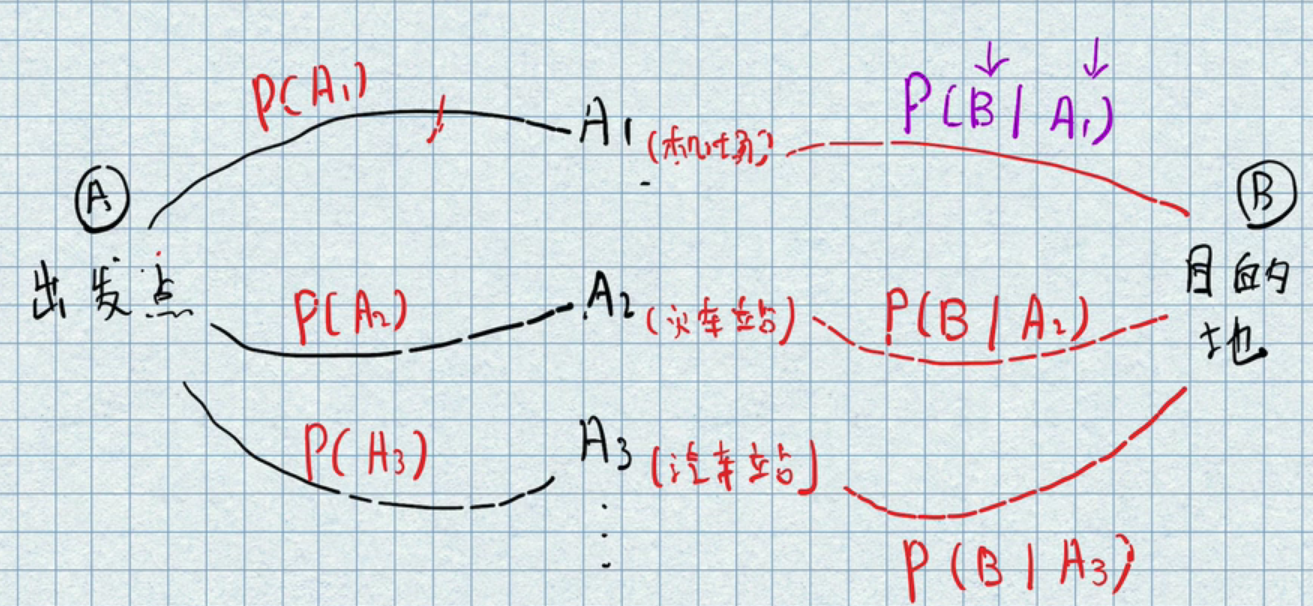
\includegraphics[scale=0.3]{1.png}}
		\end{figure}
	
		假设某人从A到B的路径有多条可以选择。则A到B的概率P为(全概率公式):
		\[p=p(A_1)p(B|A_1)+p(A_2)p(B|A_2)+p(A_3)p(B|A_3)\]
		
		若已知到达了B,推断是从哪条路线过来的?经过第一条路径到达的概率为(贝叶斯公式):
		\[p(A_1|B) = \frac{p(A_1)p(B|A_1)}{p}\]
		
		【总结】
		
		全概率公式:知因推果
		
		贝叶斯公式:知果推因
		
	\section{贝叶斯统计思想与贝叶斯估计}
		两大学派:频率学派、贝叶斯学派。频率学派只利用利用样本信息(样本观测信息)和总体信息(总体分布或总体所属分布提供的信息)。
		
		贝叶斯学派还利用了先验信息(在抽样之前有关统计问题的信息,主要时来源于经验、历史资料),对先验分布进行相应的\uline{加工},从而获得\uline{先验分布}。根据总体分布、样本信息、先验分布,得到后验分布从而进行推断。
		
		两个学派的本质区别:是否利用先验信息。
		
		【注】总体依赖于参数$\theta$的概率密度函数,在频率学派中记做$P(x;\theta)$,\uline{而在贝叶斯学派中记为}$P(x|\theta)$。
		
		\subsection{共轭先验分布}
			定义:总体分布$X~P(X|\theta)$,先验分布为$\pi(\theta)$,假如抽样后算得的后验分布$\pi(\theta|x)$与先验分布同属于一个分布族,则称先验分布$\pi(\theta)$为总体分布$X~P(X|\theta)$的一个共轭先验分布。
		\subsection{后验分布计算}
			条件概率:
			\[P(x|y) = \frac{P(x,y)}{P(y)}\]	
			
			贝叶斯公式:
			\[P(x|\theta) = \frac{P(\theta|x)P(x)}{\sum P_i}\]
			
			样本X与参数$\theta$的联合概率分布:
			\[h(X,\theta) = P(X|\theta)\cdot\pi(\theta)\]
			
			边缘密度函数:
			\[m(x) = \int_\theta h(X,\theta)d\theta = \int_\theta P(X|\theta)\cdot\pi(\theta) d\theta\] 
			 
			后验分布:
			\[\pi(\theta|x) =  \frac{h(x,\theta)}{m(x)} = \frac{P(x|\theta)\cdot \pi(\theta)}{\int_\theta P(X|\theta)\cdot\pi(\theta) d\theta}\]
			
		
			贝叶斯估计:由后验分布来估计参数$\theta$\\
			1.使用后验分布密度函数做大作为点估计,即最大后验估计。
			\[max\pi(\theta|x) = \frac{h(x,\theta)}{m(x)} = \frac{P(x|\theta)\cdot \pi(\theta)}{m(x)},\quad \propto max P(x|\theta)\cdot \pi(\theta)\]
			$m(x)$为正则化因子\\
			2.后验分布中位数\\
			3.后验分布期望
	
	\section{朴素贝叶斯分类器}
		依据贝叶斯公式计算后验概率,将后验概率最大的作为该类别。
		\[P(Y|X) = \frac{P(X|Y)\pi(Y)}{\sum P(X)}\]
		
		1.如果$\pi(Y)$未知,则假设先验概率分布是等概率。所以有
		\[maxP(Y|X)\rightarrow P(X|Y)\]
		
		2.如果$\pi(Y)$已知:$maxP(X|Y)\pi(Y)$
		
		求:
		\[P(Y|X) \quad\propto\quad P(X|Y)\pi(Y)\]
		根据条件概率公式:
		\[P(X|Y) = \frac{P(X,Y)}{P(Y)}\]
		而联合概率分布未知,所以提出\textbf{类条件独立假设}(朴素之处):即属性$x_i$之间不存在依关系。
		\[P(X|Y) = \prod_{i=1}^nP(x_i|y_i)\]
			
	\section{EM算法}
		\subsection{最大似然估计}
		最大似然估计:
		\[argmax\Big[\sum_{i=1}^NlogN(x_i|\mu,\varepsilon)\Big]\]
		分别对$\mu$和$\varepsilon$求偏导,令其导数为0,得到最优的参数。
		
		\subsection{高斯混合模型}
		高斯混合模型:两个高斯模型混合的参数$\bar{\theta}=\{\mu_1,\mu_2,\varepsilon_1,\varepsilon_2\}$。k个高斯模型的表示
		\[P(x|\bar{\theta}) = \sum_{l=1}^k\frac{1}{k}N(\mu_l,\varepsilon_l)\]
		上式将每个高斯分布同等看待,即权重都是$\frac{1}{k}$,使得组合的模型的概率分布的积分等于1。但更常见的是多个模型不等权重组合的情况。得到高斯混合模型:
		
		\begin{gather}
		P(x|\bar{\theta}) = \sum_{l=1}^k\alpha_lN(\mu_l,\varepsilon_l)\\
		\sum_{l=1}^k\alpha_l=1\\
		\bar{\theta}=\{\mu_1,\mu_2,\cdots,\mu_k,\varepsilon_1,\varepsilon_2,\cdots,\varepsilon_k,\alpha_1,\alpha_2,\cdots,\alpha_k\}
		\end{gather}
		
		在引入高斯混合模型之后,参数的最大似然估计变为:
		\[\bar{\theta}_{MLE} = argmax\Big\{\sum_{i=1}^Nlog\big[\sum_{l=1}^k\alpha_lN(\mu_l,\varepsilon_l)\big]\Big\}\]
		如果再对每个参数进行求偏导并令为0,这是很难做到的。因此需要使用迭代的算法。
		
		定义下一轮迭代的参数和上一轮的参数之间的关系为:
		\[\theta^{(g+1)} = \arg\max_{\theta}\int logP(X,Z|\theta)\cdot P(Z|X,\theta^{(g)})dZ\]
		【注】$P(X|\theta) = P_{\theta}(X)$,为两个写法。
		 
		其中Z为隐变量(latent variable),Z的加入使得简化模型的解法。
		每个样本点$x_i$的隐变量$z_i\subset \{1,2,\cdots ,k\}$,表示该样本点是属于哪个高斯分布的,因此将高斯混合模型简化为了单个的高斯模型。
		
		但是Z的加入不能改变数据的边缘分布,即要使得:
		\[P(x_i) = \int_{z_i}P_\theta(x_i|z_i)\cdot P_\theta(z_i)dz_i\]
		那么$P(z_i)$是根据高斯混合模型中的权重系数$\alpha$来的,权重越大的高斯分布,其$P(z_i)$也越大。
		\[P(z_i) = \alpha_i\]
		\[P_\theta(x_i|z_i) = N(\mu_i,\varepsilon_i)\]
		因为$z_i$都是正整数,所以积分变为求和,仍等于高斯混合模型:
		\[P(x_i) = \int_{z_i}P_\theta(x_i|z_i)\cdot P_\theta(z_i)dz_i = \sum_{i=1}^k\alpha_lN(\mu_iil,\varepsilon_i)\]
			将上式代入极大似然估计的公式中,由于log函数中是连加,所以无法得到解析解,需要用迭代算法来求解。
		\subsubsection{EM算法的有效性证明}
			EM算法:
			\[\theta^{(g+1)} = \arg\max_{\theta}\int logP(X,Z|\theta)\cdot P(Z|X,\theta^{(g)})dZ\]
			
			怎么保证迭代算法的有效性,即每一次迭代之后,似然函数要越来越大,这样才是好的。
			\[\log P(X  |\theta^{(g+1)}) \geq \log(P(X|\theta^{(g)}))\]
			所以要证明,加入了隐变量之后的迭代算法能够使得上式成立。根据条件概率公式:
			\[logP_\theta(X) = logP_\theta(X,Z) - logP_\theta(Z|X)\]
			等式两边对分布$P_{\theta^{(g)}}(Z|X)$取期望:
			\[E\big[logP_\theta(X)\big] = E\big[logP_\theta(X,Z) - logP_\theta(Z|X)\big]\]
			\[logP_\theta(X) = \int logP(X,Z|\theta)\cdot P(Z|X,\theta^{(g)})dZ-
			\int logP(Z|X,\theta)\cdot P(Z|X,\theta^{(g)})dZ \]
			
			等式右边第一项就是迭代算法需要argmax的对象,肯定是越来越大的,因此只需证明等式右边第二项会逐渐递减,则整个似然函数就会递增。令:
			\[\int logP(Z|X,\theta)\cdot P(Z|X,\theta^{(g)})dZ = H(\theta, \theta^{(g)})\]
			因此只需证明$H(\theta^{(g+1)}, \theta^{(g)}) \leq  H(\theta, \theta^{(g)})$,就能证明算法的有效性。证:
			\[H(\theta^{(g)}, \theta^{(g)}) -  H(\theta, \theta^{(g)})\geq 0\]
			
			\[
			H(\theta^{(g)}, \theta^{(g)}) -  H(\theta, \theta^{(g)})=\int logP(Z|X,\theta^{(g)})\cdot P(Z|X,\theta^{(g)})dZ-\int logP(Z|X,\theta)\cdot P(Z|X,\theta^{(g)})dZ\]
			
			\[=\int-log\Bigg(\frac{P(Z|X,\theta)}{P(Z|X,\theta^{(g)})}\Bigg)P(Z|X,\theta^{(g)})dZ
			\]

			根据琴生不等式:-log函数是凸函数,所以有(函数的期望大于期望的函数):
			\[E[f(x)]\geq f(E[x])\]
			
			\[\int-log\Bigg(\frac{P(Z|X,\theta)}{P(Z|X,\theta^{(g)})}\Bigg)P(Z|X,\theta^{(g)})dZ \\
			\geq -log\int\frac{P(Z|X,\theta)}{P(Z|X,\theta^{(g)})}P(Z|X,\theta^{(g)})dZ = -log1=0
			\]
			
			
		\subsubsection{使用EM}
			\[\theta^{(g+1)} = \arg\max_{\theta}\int logP(X,Z|\theta)\cdot P(Z|X,\theta^{(g)})dZ\]
			
			对于每一个样本点x,都有与其对应的z,而每一对$\{x_i,z_i\}$都是独立的,因此算法迭代式中的$P(X,Z|\theta)$就为:
			\[\begin{aligned}
			P(X,Z|\theta) &= \prod_{i=1}^n P(x_i,z_i|\theta) \\
			&= \prod_{i=1}^n P(x_i|z_i,\theta)P(z_i|\theta)\\
			&= \prod_{i=1}^n \alpha_{z_i} N(\mu_{z_i},\varepsilon_{z_i})
			\end{aligned}\]
			
			由于样本独立,迭代式中的另一部分可以写成:
			\[P(Z|X,\theta) = \prod_{i=1}^nP(z_i|x_i,\theta^{(g)})\]
			其中连乘的每一项表示为(全概率公式)(该样本属于某个高斯分布的概率):
			\[P(z_i|x_i,\theta)  = \frac{P(x_i|z_i)p(z_i)}{\sum_{z_{i}=1}^kP(x_i|z_i)p(z_i)}\]
			形象地表示:
			\begin{figure}[H]
				\centering{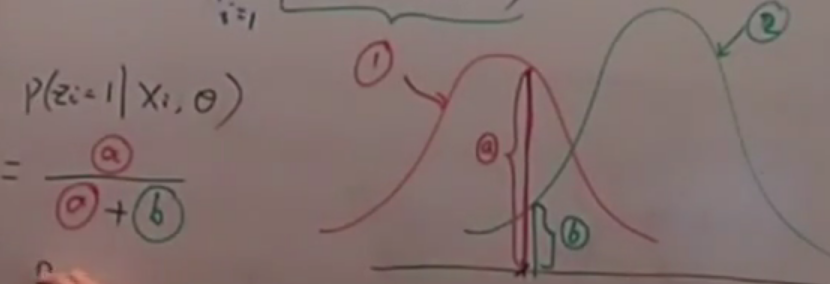
\includegraphics[scale=0.4]{3.png}}
			\end{figure}		
			将上述的两个部分带入迭代式,由于z为一系列整数,将积分换成求和。
			(N个样本,k个高斯模型)
			
			\textbf{E-step:}(求隐变量?)
			\[\sum_{z_1=1}^k\sum_{z_2=1}^k\cdots\sum_{z_N=1}^k\bigg(\sum_{i=1}^N
			\underbrace{[log\alpha_{z_i}+logN(x_i|\mu_{z_i},\varepsilon_{z_i})]}_{f_i(z_i)}
			\underbrace{\prod_{i=1}^nP(z_i|x_i,\theta^{(g)})}_{P(z_1,\cdots,z_N)}\bigg)\]
			
			\[=\sum_{z_1=1}^k\sum_{z_2=1}^k\cdots\sum_{z_N=1}^k\Big(f_1(z_1)+f_2(z_2)+\cdots +f_N(z_N)\Big)P(z_1,\cdots,z_N)\]
			
			\[=\sum_{z_1=1}^k\sum_{z_2=1}^k\cdots\sum_{z_N=1}^kf_1(z_1)P(z_1,\cdots,z_N)+\sum_{z_1=1}^k\sum_{z_2=1}^k\cdots\sum_{z_N=1}^kf_2(z_2)P(z_1,\cdots,z_N)+\cdots\]
			
			以第一项为例进行简化:
			\[\sum_{z_1=1}^k\sum_{z_2=1}^k\cdots\sum_{z_N=1}^kf_1(z_1)P(z_1,\cdots,z_N) = \sum_{z_1=1}^kf_1(z_1)\cdot \underbrace{\sum_{z_2=1}^k\cdots\sum_{z_N=1}^kP(z_1,\cdots,z_N)}_{P(z_1)\text{的边缘分布}}\]
			\[=\sum_{z_1=1}^kf_1(z_1)P(z_1)\]
			
			所以E-step的步骤可以简化为: 
			\[\sum_{i=1}^N\sum_{z_i=1}^k\Big(log\alpha_{z_i}+logN(x_i|\mu_{z_i},\varepsilon_{z_i})\Big) P(z_i|x_i,\theta^{(g)})\]
			
			\[\theta^{(g+1)} =\arg\max_{\theta} \sum_{i=1}^N\sum_{z_i=1}^k\Big(log\alpha_{z_i}+logN(x_i|\mu_{z_i},\varepsilon_{z_i})\Big)\underbrace{\frac{P(x_i|z_i)p(z_i)}{\sum_{z_{i}=1}^kP(x_i|z_i)p(z_i)}}_{P(z_i|x_i,\theta^{(g)})}\]
			
			\textbf{M-step:}
			
			分别对$\alpha$和$\mu,\varepsilon$求偏导,并令其等于0,取极大值。
			
			\uline{首先对$\alpha$求偏导使得:}
			\[\frac{\partial\sum_{i=1}^N\sum_{z_i=1}^klog\alpha_{z_i}P(z_i|x_i,\theta^{(g)})}{\partial\alpha_1,\cdots,\partial\alpha_k} = [0\cdots0],\quad s.t.\sum_{z_i=1}^k\alpha_{z_i}=1\]
			
			这是一个带约束条件的优化问题,利用拉格朗日乘数法来求解:
			\[L(\alpha_1,\alpha_2,\cdots,\alpha_k,\lambda) = \sum_{z_i=1}^klog\alpha_{z_i}\Bigg(\sum_{i=1}^NP(z_i|x_i,\theta^{(g)})\Bigg) +\lambda\Bigg(\sum_{z_i=1}^k\alpha_{z_i}-1\Bigg)\]
			
			\[\Longrightarrow \frac{\partial L}{\partial\alpha_i}  = \frac{1}{\alpha_i}\Bigg(\sum_{i=1}^NP(z_i|x_i,\theta^{(g)})\Bigg)+\lambda =0 \]
			
			\[\Longrightarrow\sum_{i=1}^NP(z_i|x_i,\theta^{(g)}) +\alpha_i\lambda=0\]
			
			利用约束条件$\sum_{z_i=1}^k\alpha_{z_i}=1$,求和:
			\[\Longrightarrow\sum_{i=1}^N\underbrace{\sum_{z_i=1}^kP(z_i|x_i,\theta^{(g)})}_{=1} +\underbrace{\sum_{z_i=1}^k\alpha_i}_{=1}\lambda=0\]
			
			\[\Longrightarrow N+\lambda =0, \quad \lambda=-N\]
			
			将$\lambda$代入可得:				
			\[\Longrightarrow \alpha_i = \frac{1}{N}\sum_{i=1}^NP(z_i|x_i,\theta^{(g)}) = \frac{1}{N}\sum_{i=1}^N\frac{p(z_i)N(x_i|\theta^{(g)})}{\sum_{z_{i}=1}^kp(z_i)N(x_i|\theta^{(g)}}\]
			
			\uline{对均值求偏导并置之为零:}
			
			二维的高斯分布公式:
			\[N(\bm{x}|\bm{\mu},\bm{\Sigma}) = \frac{1}{2\pi|\bm{\Sigma}|^{\frac{1}{2}}}exp[-\frac{1}{2}(\bm{x}-\bm{\mu})^T\bm{\Sigma}^{-1}(\bm{x}-\bm{\mu})]\]
			
			其中向量$\bm{x}=[x,y]$表示样本的坐标,$\bm{\mu}=[x_0,y_0]$为高斯分布的均值,$\bm{\Sigma}$为二维随机变量x,y的协方差矩阵。
			
			去除无关项,并代入高斯分布函数:
			\[F = \sum_{i=1}^N\sum_{z_i=1}^k\Big(log\frac{1}{2\pi|\bm{\Sigma}|^{\frac{1}{2}}}-\frac{1}{2}(\bm{x}-\bm{\mu})^T\bm{\Sigma}^{-1}(\bm{x}-\bm{\mu}))\Big)
			P(z_i|x_i,\theta^{(g)})\]
			
			\textbf{对$\bm{\mu}_{z_i}$求导:}
			\[\frac{\partial F}{\partial \bm{\mu}_{z_i}} = \sum_{i=1}^N\bm{\Sigma}_{z_i}^{-1}(\bm{x}_i-\bm{\mu}_{z_i})\underbrace{P(z_i|x_i,\theta^{(g)})}_{\text{常量}}=0\]
			两边同时乘以$\bm{\Sigma}_{z_i}$(假设协方差矩阵非奇异),解得:
				\[\bm{\mu}_{z_i} = \sum_{i=1}^N\frac{1}{P(z_i|x_i,\theta^{(g)})} \sum_{i=1}^{N}P(z_i|x_i,\theta^{(g)})\bm{x}_i\]
				
			\textbf{对$\bm{\Sigma}_{z_i}$求导,}并置为零,解得:
			\[\bm{\Sigma}_{z_i} = \sum_{i=1}^N\frac{1}{P(z_i|x_i,\theta^{(g)})} \sum_{i=1}^{N}P(z_i|x_i,\theta^{(g)})(\bm{x}_i-\bm{\mu}_{z_i})(\bm{x}_i-\bm{\mu}_{z_i})^T\]
				
				
			
		
			
			
\end{document}